\section{Методы оптимизации}

Напомним, что рассматривается задача поиска минимума величины $Q(x) \textrm{, где } x=(x_1 \dots x_n) \textrm{, при этом } Q(x) \geq 0 \textrm{ в области } U \in \mathbb{R}^n$. Предполагается, что этот минимум лежит внутри области $U$. В действительности мы ищем \textbf{локальные минимумы} $Q(x)$, которых может быть несколько. Абсолютный минимум находится путем сравнения локальных.

Подчеркнем, что все описанные ниже алгоритмы поиска локальных минимумов можно использовать и для решения системы нелинейных уравнений вида $f(x) = 0$ (\ref{eq:7.9}).

Ниже будут описаны алгоритмы \textbf{покоординатного} и \textbf{градиентного} спусков. Эти алгоритмы содержатся в любом пакете прикладных программ. Кроме того, будет кратко описан \textbf{метод оврагов}, предложенный И. М. Гельфандом и его сотрудниками.

Начнем с \textbf{покоординатного спуска}. В сущности это описанный выше метод редукции к одномерному случаю. Для реализации покоординаного спуска снова выбирается нулевое приближение $x^{(0)} = (x^{(0)}_1 \dots x^{(0)}_n)$. Уравнения $x_2 = x_2^{(0)} \dots x_n^{(0)} = x_n^{(0)}$ задают прямую в $\mathbb{R}^n$. На этой прямой ищется минимум величины $Q(x)$ по переменной $x_1$. Это дает величины $x^{(1)}_1$. Величина $x^{(0)}_2$ определяется как минимум $Q(x)$ на прямой $x_1 = x_1^{(1)}, x_3 = x_3^{(0)} \dots x_n = x_n^{(0)}$ и так далее. В методе координатного спуска, так же как и при решении системы уравнений $f(x) = 0$, возникает проблема выбора приближения $x^{(0)}$. 

Чтобы проиллюстрировать возникающие трудности, рассмотрим двумерный случай. Пусть $x = x_1 \textrm{ и } y=x_2$. Чтобы локализовать минимумы величны $Q(x, y)$, полезно нарисовать карту, на которой горизонтали это линии уровней (кривые, на которых $Q(x, y) = c_i$). На рисунке \ref{fig:map} представлена карта с двумя минимумами в точках $(x_0, y_0), (\tilde x_0, \tilde y_0)$.


%%%figure_map_not_done

%%%figure_map_not_done


Для сходимости алгоритма точку $(x^{(0)}, y^{(0)})$ необходимо выбрать так, чтобы кривые $Q(x, y) = c_i \textrm{ при } c_i < Q(x^{(0)}, y^{(0)})$ имели вид "эллипсов".

При таком выборе точки $(x^{(0)}, y^{(0)})$  схема действия алгоритма покоординатного спуска представлена на рисунке \ref{fig:coordinate_descent}.


%%%%figure_coordinate_descent_done
\begin{figure}[h] % picture
	\centering
	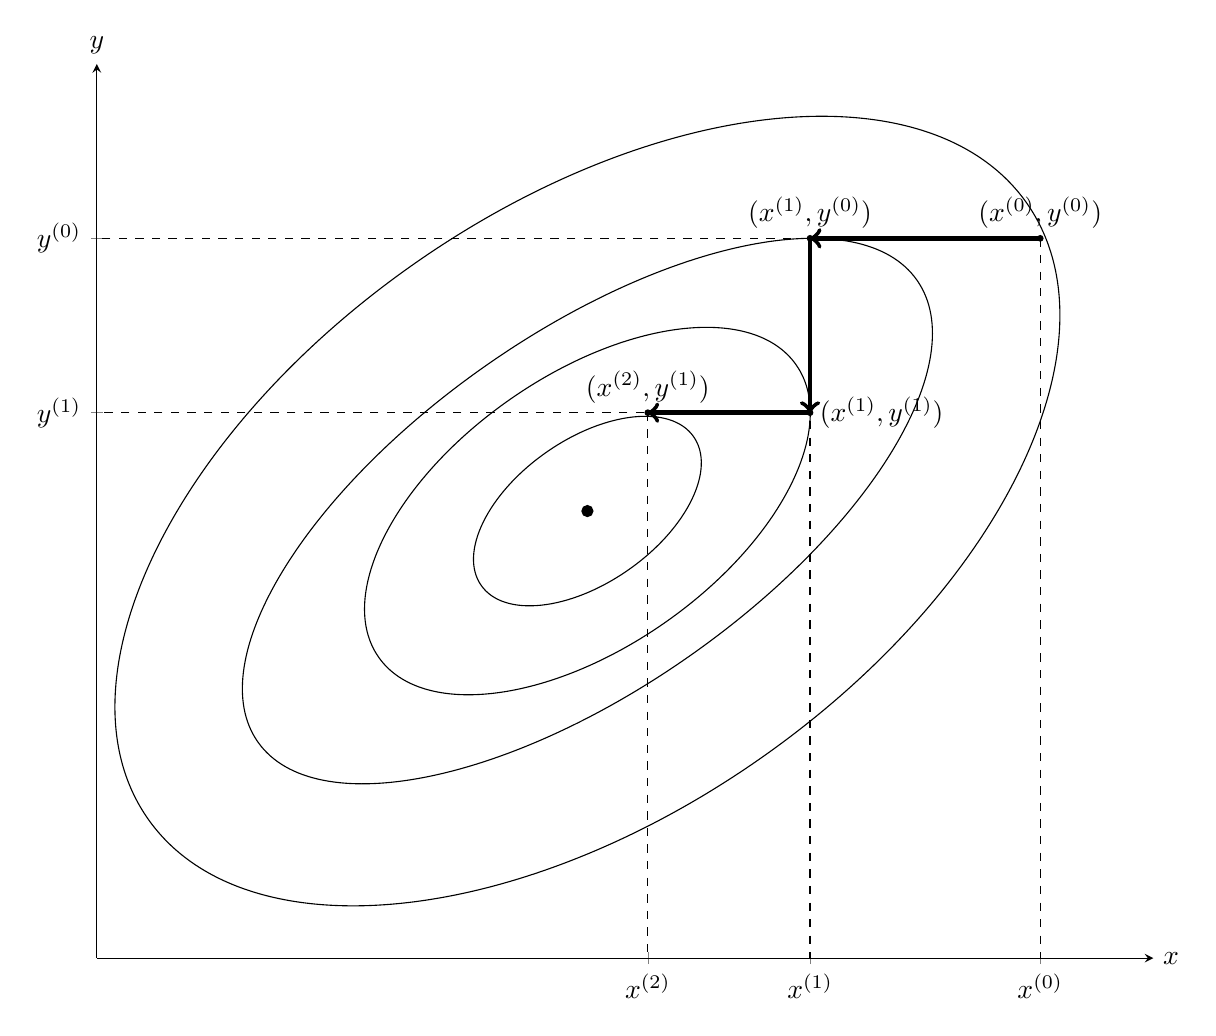
\begin{tikzpicture}
\begin{axis}[
	width = 15cm,
	xmin=-13,   xmax=15,
	ymin=-10,   ymax=10,
	axis y line*=left,
    axis x line*=bottom,
    axis lines = left,
	xtick={12, 5.9, 1.6},
	xticklabels = {$x^{(0)}$, $x^{(1)}$,$x^{(2)}$},
	ytick={6.1, 2.2},
	yticklabels = {$y^{(0)}$, $y^{(1)}$},
	        ylabel = {$y$}, ylabel style={rotate=-90},
        xlabel = {$x$},
        every axis x label/.style={
    		at={(ticklabel* cs:1.0)},
   			anchor=west,
			},
		every axis y label/.style={
    		at={(ticklabel* cs:1.0)},
    		anchor=south,
			}
]


	\draw[rotate around={-55:(0,0)},black] (0,0) ellipse (8 and 12);
	\draw[rotate around={-55:(0,0)},black] (0,0) ellipse (4.7 and 9);
	\draw[rotate around={-55:(0,0)},black] (0,0) ellipse (3.6 and 5.7);
	\draw[rotate around={-55:(0,0)},black] (0,0) ellipse (1.9 and 2.9);
	
	\addplot [only marks,mark=*] coordinates { (0,0) };

    
	\coordinate[label=above:{$(x^{(0)}, y^{(0)})$}] (A) at (12, 6.1);
	
	\draw[fill] (A) circle (1pt);
	\draw [dashed] (A) -- (A |- 0,-10);
	\draw [dashed] (A) -- (A -| -13,0);
	
	\coordinate[label=above:{$(x^{(1)}, y^{(0)})$}] (B) at (5.9, 6.1);
	
	\draw[fill] (B) circle (1pt);
	\draw [dashed] (B) -- (B |- 0,-10);
%	\draw [dashed] (B) -- (B -| -13,0);
	
	\coordinate[label=right:{$(x^{(1)}, y^{(1)})$}] (C) at (5.9, 2.2);
	
	\draw[fill] (C) circle (1pt);
%	\draw [dashed] (C) -- (C |- 0,-10);
	\draw [dashed] (C) -- (C -| -13,0);
	
	\coordinate[label=above:{$(x^{(2)}, y^{(1)})$}] (D) at (1.6, 2.2);
	
	\draw[fill] (D) circle (1pt);
	\draw [dashed] (D) -- (D |- 0,-10);
	
	\draw [->, ultra thick] (A) -- (B);
	\draw [->, ultra thick] (B) -- (C);
	\draw [->, ultra thick] (C) -- (D);
	
\end{axis}
\end{tikzpicture}

	\caption{Координатный спуск.}
	\label{fig:coordinate_descent}

\end{figure}
%%%%figure_coordinate_descent_done


При поиске $x^{(1)}$ мы движемся по прямой $y = y^{(0)}$ до тех пор, пока эта прямая не коснется некоторой линии уровня и так далее.

Алгоритм покоординатного спуска быстро сходится, если "эллипс" $Q(x, y) = c_i \textrm{ при } c_i < Q(x^{(0)}, y^{(0)})$ близки к кругам. Этот алгоритм сходится медленно, если "эллипсы" сильно вытянуты вдоль оси не параллельной осям координат. В этом случае полезно перейти к координатам в которых оси "эллипсов" параллельны осям координат.

Однако лучше использовать \textbf{градиентный спуск}. В этом методе прямая, вдоль которой ищется минимум $Q(x, y)$, выбирается независимо от выбора осей координат.

Для формулировки алгоритма градиентного спуска надо ввести понятие \textbf{градиента функции $Q(x)$}, где $x = (x_1 \dots x_n)$. Это вектор $\nabla Q(x)$
\begin{equation} \label{eq:8.1}
	\nabla Q(x) = (\frac{\partial Q}{x_i}(x) \dots \frac{\partial Q}{x_i}(x))
\end{equation}
Поясним геометрический смысл вектора $\nabla Q(x)$. Единичный вектор $\xi = (\xi_1 \dots \xi_n), \|\xi\| = 1$ задает некоторое направление в $\mathbb{R}^n$. Введем величину $\nabla_\xi Q$ - производную $Q(x)$ по направлению $\xi$
\begin{equation} \label{eq:8.2}
	\nabla_\xi Q(x) = \lim_{\varepsilon \to 0} \frac{Q(x+\varepsilon\xi) - Q(x)}{\varepsilon}
\end{equation}
Так как
\begin{equation} \label{eq:8.3}
	Q(x+\varepsilon\xi) = Q(x) + \varepsilon\sum^n_{i=1}{\xi_i \frac{\partial Q}{\partial x_i}(x) + \mathcal{O}(\varepsilon^2)} = Q(x) + \varepsilon(\nabla Q(x), \xi) + \mathcal{O}(\varepsilon^2),
\end{equation}
то отсюда следует, что
\begin{equation} \label{eq:8.4}
	\nabla_\xi Q(x) = (\nabla Q(x), \xi) 
\end{equation}
Вектор $\nabla Q$ задает направление $\xi_0$
\begin{equation} \label{eq:8.5}
	\nabla Q = \|\nabla Q(x)\|\xi_0 
\end{equation}
и следовательно
\begin{equation} \label{eq:8.6}
	\nabla_\xi Q(x) = \|\nabla Q(x)\|(\xi, \xi_0) 
\end{equation}
Таким образом, $\xi_0$ - это направление, вдоль которого величина $Q(x)$ меняется наиболее быстро, и вектор $\nabla Q(x)$ направлен по нормали к поверхности уровня $Q(x) = C$.

Алгоритм градиентного спуска действует следующим образом. Пусть задано нулевое приближение $x^{(0)} \in \mathbb{R}^n$. Определим функцию $\varphi_0(t) (t \in \mathbb{R}^1)$ равенством
\begin{equation} \label{eq:8.7}
	\varphi_0(t) = Q(x^{(0)} - t\nabla Q(x^{(0)})) 
\end{equation}
и найдем $t_0$ из условия $\varphi_0(t) = min$. Тогда
\begin{align}
	\begin{split} \label{eq:8.8}
		x^{(1)} = x^{(0)} - t_0\nabla Q(x^{(0)}) \\
		x^{(2)} = x^{(1)} - t_1\nabla Q(x^{(1)}),
	\end{split}
\end{align}
где $t_1$ точки минимума функции
\begin{equation} \label{eq:8.9}
	\varphi_1(t) = Q(x^{(1)} - t\nabla Q(x^{(1)})) \textrm{ и так далее}
\end{equation}

Схема действия алгоритма градиентного спуска в двумерном случае $(x_1 = x, x_2 = y)$ показана на рисунке \ref{fig:2d_gradient}.


%%%%figure_2d_gradient_done
\begin{figure}[h] % picture
	\centering
	\begin{tikzpicture}
	\begin{axis}[
	width = 15cm,
	xmin=-13,   xmax=13,
	ymin=-10,   ymax=10,
	axis y line*=left,
	axis x line*=bottom,
	axis lines = left,
	domain=0:30,
	xtick={7.9, 1.9, -1.1},
	xticklabels = {$x^{(0)}$, $x^{(1)}$,$x^{(2)}$},
	ytick={7, 1, 4},
	yticklabels = {$y^{(0)}$, $y^{(1)}$, $y^{(2)}$},
	ylabel = {$y$}, ylabel style={rotate=-90},
	xlabel = {$x$},
	every axis x label/.style={
		at={(ticklabel* cs:1.0)},
		anchor=west,
	},
	every axis y label/.style={
		at={(ticklabel* cs:1.0)},
		anchor=south,
	}
	]
	
	\coordinate (O) at (-0.7, 2.8);
	\coordinate (O1) at (-2.1, 3.1);
	
	\draw[rotate around={-45:(0,0)},black] (0,0) ellipse (8 and 10);
	\draw[rotate around={-45:(O)},black] (O) ellipse (3.2 and 4);
	\draw[rotate around={-45:(O1)},black] (O1) ellipse (1 and 1.25);
	%	
	%	\draw[fill] (0, 0) circle (1pt);
	%
	
	\coordinate[label=right:{$(x^{(0)}, y^{(0)})$}] (A) at (7.9, 7);
	\draw[fill] (A) circle (1pt);
	
	\addplot[dashed] {-x + 14.9}; % perpendicular is x
	
	\coordinate[label=right:{$(x^{(1)}, y^{(1)})$}] (B) at (1.9, 1);
	\draw[fill] (B) circle (1pt);
	
	\draw[dashed] (A) -- (-0.1, -1); 
	
	\coordinate[label=right:{$(x^{(2)}, y^{(2)})$}] (C) at (-1.1, 4);
	\draw[fill] (C) circle (1pt);
	
	\draw[dashed] (B) -- (-3.1, 6); 

		
  	\draw[->, ultra thick] (A) -- (B);
  	\draw[->, ultra thick] (B) -- (C);
  	
  	
  	\draw [dashed] (A) -- (A |- 0,-10);

	\draw [dashed] (A) -- (A -| -13,0);
	
	\draw [dashed] (B) -- (B |- 0,-10);
	\draw [dashed] (B) -- (B -| -13,0);
	
	\draw [dashed] (C) -- (C |- 0,-10);
	\draw [dashed] (C) -- (C -| -13,0);
	

\end{axis}
\end{tikzpicture}
	\caption{Градиентный спуск.}
	\label{fig:2d_gradient}
\end{figure}
%%%%figure_2d_gradient_done


Как правило, алгоритм градиентного спуска работает существенно быстрее алгоритма покоординатного спуска. Однако, если карта уровней $Q(x, y) = c_i$ выглядит как показано на рисунке \ref{fig:map_weird}, то оба описанных выше алгоритма сходятся очень медленно.


%%%figure_map_weird_not_done

%%%figure_map_weird_not_done


И. М. Гельфанд с сотрудниками предложили \textbf{метод оврагов}, который и в этом случае быстро находит дно оврага - точку $(x_0, y_0)$. Идея состоит в том, что исходной является не одна точка $(x^{(0)}, y^{(0)})$, а две $(x^{(0)}_1, y^{(0)}_1), (x^{(0)}_2, y^{(0)}_2)$. Схема этого метода представлена на рисунке \ref{fig:ravine_method}.


%%%figure_ravine_method_not_done

%%%figure_ravine_method_not_done




\begin{figure}[h] % picture
	\centering
	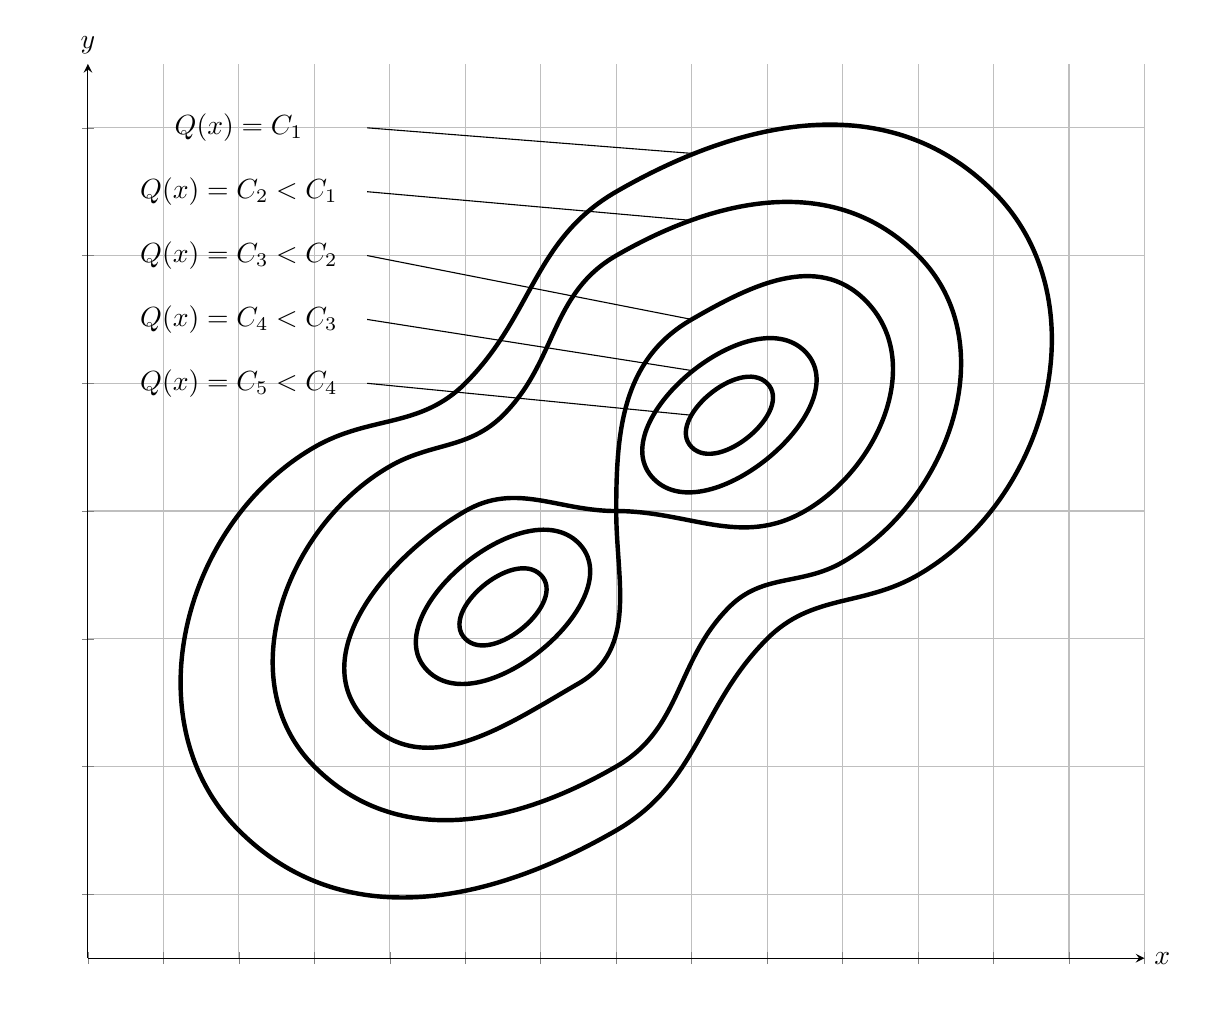
\begin{tikzpicture}
	
	\begin{axis}[
	width = 15cm,
	xmin=-7,   xmax=7,
	ymin=-7,   ymax=7,
	axis y line*=left,
    axis x line*=bottom,
    axis lines = left,
    domain=0:30,
    grid = major,
    tick label style = {white},
		    ylabel = {$y$}, ylabel style={rotate=-90},
        xlabel = {$x$},
        every axis x label/.style={
    		at={(ticklabel* cs:1.0)},
   			anchor=west,
			},
		every axis y label/.style={
    		at={(ticklabel* cs:1.0)},
    		anchor=south,
			}
]
 \draw [ultra thick,black] (5, 5 ) to[out=-45,in=30] (4, -1)
 		to[out=-150,in=45] (2,-2) to[out=-135,in=30] (0, -5)
 		to[out=-150,in=-45] (-5, -5)  to[out=135,in=-150] (-4, 1) 
 		to[out=30,in=-135] (-2, 2)  to[out=45,in=-150] (0, 5)
 		to[out=30,in=135] (5, 5) ;
 \draw [ultra thick,black] (4, 4 ) to[out=-45,in=30] (3, -0.8)
 		to[out=-150,in=45] (1.5,-1.5) to[out=-135,in=30] (0, -4)
 		to[out=-150,in=-45] (-4, -4)  to[out=135,in=-150] (-3, 0.7) 
 		to[out=30,in=-135] (-1.5, 1.5)  to[out=45,in=-150] (0, 4)
 		to[out=30,in=135] (4, 4)  ;
 \draw [ultra thick,black] (3.3, 3.3 ) to[out=-45,in=30] (2.5, 0)
 		to[out=-150,in=0] (0, 0)  to[out=90,in=-150] (1, 3)
 		to[out=30,in=135] (3.3,3.3)  ;
  \draw [ultra thick,black] (-3.3, -3.3 ) to[out=135,in=-150] (-2, 0)
 		to[out=30,in=180] (0, 0)  to[out=-90,in=30] (-0.5, -2.7)
 		to[out=-150,in=-45] (-3.3, -3.3) ;
 \draw [ultra thick,black] (2.5, 2.5) to[out=-45,in=-45] (0.5, 0.5) to[out=135,in=135] (2.5,2.5 );
  \draw [ultra thick,black] (2, 2) to[out=-45,in=-45] (1, 1) to[out=135,in=135] (2,2 );
  \draw [ultra thick,black] (-2.5, -2.5) to[out=-45,in=-45] (-0.5, -0.5) to[out=135,in=135] (-2.5,-2.5 );
  \draw [ultra thick,black] (-2, -2) to[out=-45,in=-45] (-1, -1) to[out=135,in=135] (-2,-2 );
  
  \node (A) at (-5, 6) {$Q(x) = C_1$};
  \draw (-3.3, 6) -- (1, 5.6);
  \node (B) at (-5, 5) {$Q(x) = C_2 < C_1$};
  \draw (-3.3, 5) -- (1, 4.55);
  \node (C) at (-5, 4) {$Q(x) = C_3 < C_2$};
  \draw (-3.3, 4) -- (1, 3.0);
  \node (D) at (-5, 3) {$Q(x) = C_4 < C_3$};
  \draw (-3.3, 3) -- (1, 2.2);
  \node (E) at (-5, 2) {$Q(x) = C_5 < C_4$};
  \draw (-3.3, 2) -- (1, 1.5);
\end{axis}
		
	\end{tikzpicture}
	\caption{Сложный ландшафт.}
	\label{fig:complex_landscape}
\end{figure}





\begin{figure}[h] % picture
	\centering
	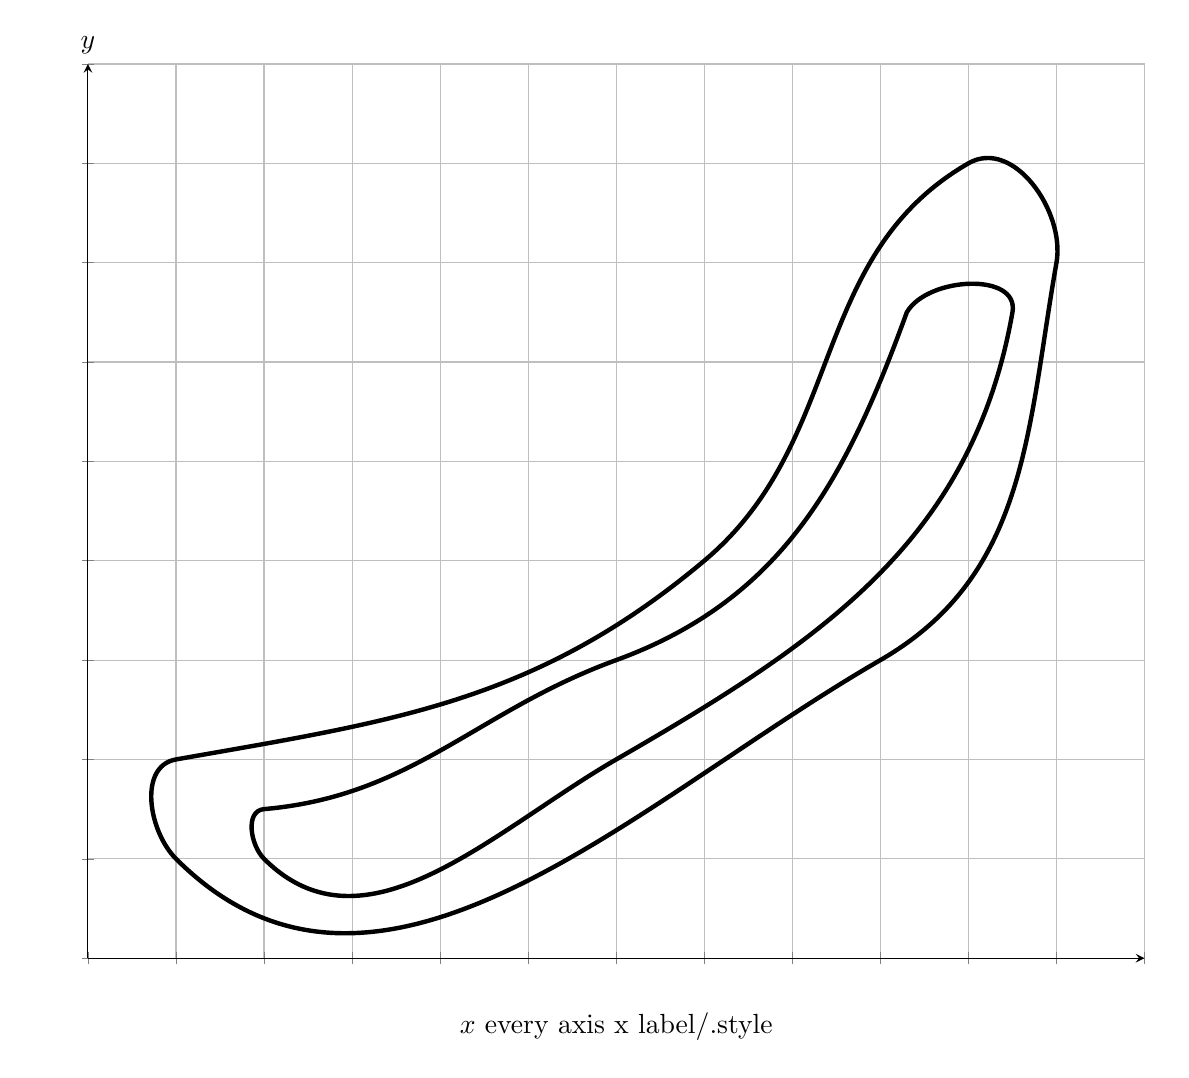
\begin{tikzpicture}
	
	\begin{axis}[
	width = 15cm,
	xmin=-5,   xmax=7,
	ymin=-2,   ymax=7,
	axis y line*=left,
    axis x line*=bottom,
    axis lines = left,
    domain=0:30,
    tick label style = {white},
    grid = major,
	    ylabel = {$y$}, ylabel style={rotate=-90},
        xlabel = {$x$}
        every axis x label/.style={
    		at={(ticklabel* cs:1.0)},
   			anchor=west,
			},
		every axis y label/.style={
    		at={(ticklabel* cs:1.0)},
    		anchor=south,
			}
]
 
 \draw [ultra thick,black] (-4, -1 ) to[out=-45,in=-150] (4, 1) to[out=30,in=-100] (6, 5)  to[out=80,in=30] (5, 6) to[out=-150,in=40] (2, 2) to[out=-140,in=10] (-4, 0) to[out=-170,in=135] (-4, -1)	 
 ;
 
 \draw [ultra thick,black] (-3, -1 ) to[out=-45,in=-150] (1, 0) to[out=30,in=-100] (5.5, 4.5)  to[out=80,in=60] (4.3, 4.5) to[out=-110,in=20] (1, 1) to[out=-160,in=5] (-3, -0.5) to[out=-175,in=135] (-3, -1)	 
 ;
		
\end{axis}
	\end{tikzpicture}
	\caption{Овраг}
	\label{fig:ovrag}
\end{figure}






